\chapter{Link Loss vs Noise}
\label{ch:link-loss-vs-noise}

\begin{nontechnical}
\textbf{Link loss vs noise is like the difference between someone whispering (weak signal) vs shouting in a loud room (noise interference)---two different problems!}

\textbf{Link Loss} - Signal gets weaker:
\begin{itemize}
\item \textbf{What it is}: Your WiFi router is far away, so signal is weak by the time it reaches you
\item \textbf{Analogy}: Shouting across a football field---your voice spreads out and gets quieter
\item \textbf{Predictable}: Same distance = same loss every time
\item \textbf{Solution}: Move closer, use bigger antenna, increase transmit power
\end{itemize}

\textbf{Examples of link loss}:
\begin{itemize}
\item \textbf{WiFi}: 50 meters away = 10,000$\times$ weaker signal
\item \textbf{Cell phone}: Far from tower = fewer bars
\item \textbf{Satellite}: Space is far! Signal arrives incredibly weak
\end{itemize}

\textbf{Noise} - Random interference added:
\begin{itemize}
\item \textbf{What it is}: Random electrical static from electronics, thermal energy, cosmic rays
\item \textbf{Analogy}: Trying to hear someone whisper in a noisy restaurant---extra sound covers the signal
\item \textbf{Random}: Unpredictable, changes moment-to-moment
\item \textbf{Solution}: Can't remove it! Must send stronger signal or use error correction
\end{itemize}

\textbf{Examples of noise}:
\begin{itemize}
\item \textbf{Bluetooth stuttering near microwave}: Microwave adds noise
\item \textbf{AM radio crackle}: Thunderstorms add noise
\item \textbf{TV static}: No signal? You're seeing pure noise!
\end{itemize}

\textbf{Key difference}:
\begin{itemize}
\item \textbf{Link loss}: Makes signal weaker (deterministic, predictable)
\item \textbf{Noise}: Adds random garbage on top (random, unpredictable)
\item \textbf{Both hurt you}: Weak signal (loss) covered by noise = errors!
\end{itemize}

\textbf{The engineering ratio: SNR (Signal-to-Noise Ratio)}
\begin{itemize}
\item Strong signal + low noise = high SNR = perfect communication
\item Weak signal (loss) + high noise = low SNR = errors everywhere
\end{itemize}

\textbf{Real-world example}: Your phone shows ``5 bars'' (link loss is low) but internet is slow (noise is high from interference).
\end{nontechnical}

\section{Overview}

In a real communication system, the received signal is degraded by \textbf{two distinct mechanisms}: link loss and additive noise. Understanding the difference is crucial for link budget analysis and system design.

\begin{keyconcept}
\textbf{Link loss} is deterministic and multiplicative---it reduces signal power predictably. \textbf{Noise} is random and additive---it adds unpredictable interference. Both degrade performance, but in fundamentally different ways requiring different mitigation strategies.
\end{keyconcept}

The relationship between link loss, noise, and system performance is captured by the signal-to-noise ratio (SNR), which determines the achievable bit error rate (BER) for a given modulation scheme.

\section{Mathematical Description}

\subsection{System Model}

The complete channel can be modeled as a cascade of deterministic attenuation followed by additive noise:

\begin{center}
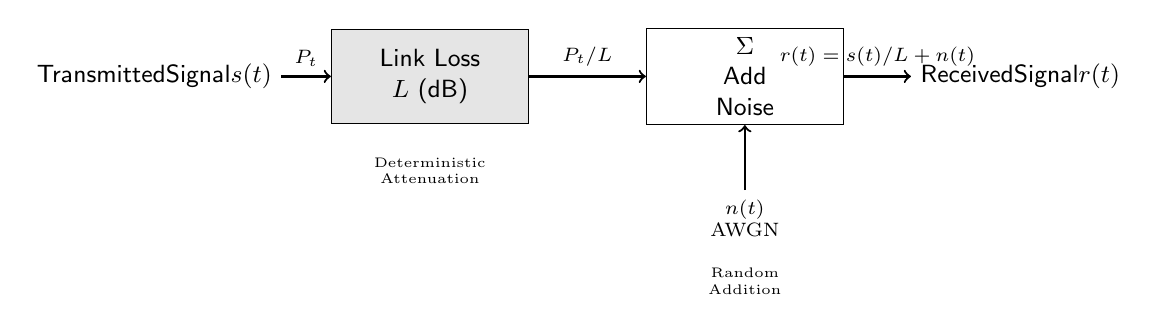
\begin{tikzpicture}[
  block/.style={rectangle, draw, minimum width=2.5cm, minimum height=1.2cm, font=\sffamily\small, align=center},
  node distance=3cm,
  font=\small
]
\node (input) {\sffamily Transmitted\\Signal\\$s(t)$};
\node[block, right of=input, node distance=3.5cm, fill=black!10] (loss) {Link Loss\\$L$ (dB)};
\node[block, right of=loss, node distance=4cm] (adder) {$\Sigma$\\Add\\Noise};
\node[right of=adder, node distance=3.5cm] (output) {\sffamily Received\\Signal\\$r(t)$};

\node[below of=adder, node distance=1.8cm, font=\scriptsize, align=center] (noise) {$n(t)$\\AWGN};

\draw[->,thick] (input) -- node[above,font=\scriptsize] {$P_t$} (loss);
\draw[->,thick] (loss) -- node[above,font=\scriptsize] {$P_t/L$} (adder);
\draw[->,thick] (noise) -- (adder);
\draw[->,thick] (adder) -- node[above,font=\scriptsize] {$r(t) = s(t)/L + n(t)$} (output);

% Power annotations
\node[below of=loss, node distance=1.2cm, font=\tiny, align=center] {Deterministic\\Attenuation};
\node[below of=noise, node distance=0.8cm, font=\tiny, align=center] {Random\\Addition};
\end{tikzpicture}
\end{center}

The received signal is expressed as:
\begin{equation}
r(t) = \frac{s(t)}{\sqrt{L}} + n(t)
\end{equation}
where:
\begin{itemize}
\item $s(t)$ = transmitted signal (watts)
\item $L$ = link loss factor (dimensionless, $> 1$)
\item $n(t)$ = additive white Gaussian noise (watts)
\item $r(t)$ = received signal (watts)
\end{itemize}

\subsection{Link Loss (Path Loss)}

\textbf{Link Loss} represents the deterministic reduction in signal power as it travels from transmitter to receiver.

\subsubsection{Characteristics}

\begin{itemize}
\item \textbf{Deterministic}: Same loss every time (for a given scenario)
\item \textbf{Multiplicative}: Scales the entire signal uniformly
\item \textbf{Predictable}: Can be calculated from path distance, frequency, antenna gains
\item \textbf{Independent of signal content}: Affects all signals equally
\end{itemize}

\subsubsection{Sources of Link Loss}

Link loss arises from multiple contributors in the propagation path:

\begin{center}
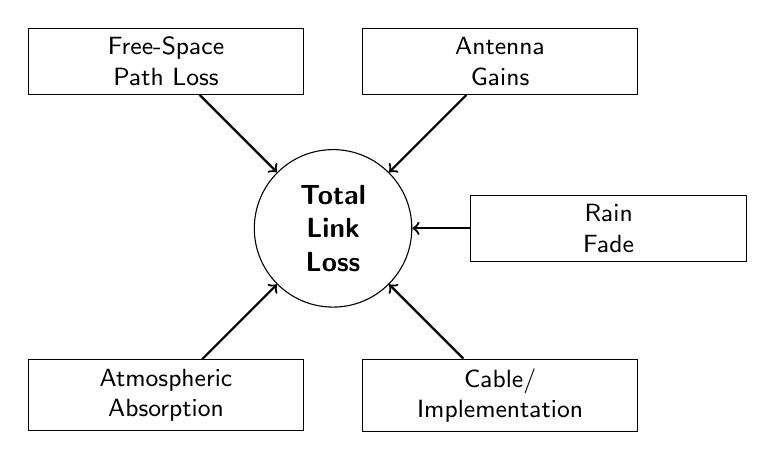
\begin{tikzpicture}[
  node distance=1.5cm and 2cm,
  block/.style={rectangle, draw, minimum width=3.5cm, minimum height=0.8cm, font=\sffamily\small, align=center},
  font=\small
]
% Central node
\node[circle, draw, minimum size=2cm, font=\bfseries\sffamily, align=center] (center) {Total\\Link\\Loss};

% Surrounding nodes
\node[block, above left of=center, node distance=3cm] (fspl) {Free-Space\\Path Loss};
\node[block, above right of=center, node distance=3cm] (antenna) {Antenna\\Gains};
\node[block, below left of=center, node distance=3cm] (atmos) {Atmospheric\\Absorption};
\node[block, below right of=center, node distance=3cm] (cable) {Cable/\\Implementation};
\node[block, right of=center, node distance=3.5cm] (rain) {Rain\\Fade};

% Arrows
\draw[->,thick] (fspl) -- (center);
\draw[->,thick] (antenna) -- (center);
\draw[->,thick] (atmos) -- (center);
\draw[->,thick] (cable) -- (center);
\draw[->,thick] (rain) -- (center);
\end{tikzpicture}
\end{center}

\textbf{Primary contributors}:
\begin{itemize}
\item \textbf{Free-space path loss}: Geometric spreading of energy ($\propto d^2$)
\item \textbf{Antenna gains}: TX and RX antenna directivity (can be gain or loss)
\item \textbf{Cable losses}: Attenuation in feedlines and connectors
\item \textbf{Atmospheric absorption}: Molecular absorption (O$_2$, H$_2$O)
\item \textbf{Rain attenuation}: Scattering and absorption by hydrometeors
\end{itemize}

\subsubsection{Mathematical Model}

In linear scale, link loss is multiplicative:
\begin{equation}
P_{\text{rx}} = \frac{P_{\text{tx}}}{L}
\end{equation}
where:
\begin{itemize}
\item $P_{\text{rx}}$ = received power (watts)
\item $P_{\text{tx}}$ = transmitted power (watts)
\item $L$ = total link loss factor (dimensionless, $L > 1$)
\end{itemize}

In logarithmic (dB) scale, link loss is subtractive:
\begin{equation}
P_{\text{rx}}\ [\text{dBm}] = P_{\text{tx}}\ [\text{dBm}] - L_{\text{dB}}\ [\text{dB}]
\end{equation}
where:
\begin{itemize}
\item $L_{\text{dB}} = 10\log_{10}(L)$ = link loss in decibels
\end{itemize}

\textbf{Free-space path loss (FSPL)} is the dominant component:
\begin{equation}
L_{\text{FSPL}}\ [\text{dB}] = 20\log_{10}(d) + 20\log_{10}(f) + 20\log_{10}\left(\frac{4\pi}{c}\right)
\end{equation}
where:
\begin{itemize}
\item $d$ = distance (meters)
\item $f$ = frequency (Hz)
\item $c = 3 \times 10^8$ m/s (speed of light)
\end{itemize}

Simplified form:
\begin{equation}
L_{\text{FSPL}}\ [\text{dB}] = 20\log_{10}(d_{\text{km}}) + 20\log_{10}(f_{\text{MHz}}) + 32.45
\end{equation}

\subsubsection{Link Budget Example}

\begin{calloutbox}{Example: Simple Link Budget}
\begin{tabular}{@{}lr@{}}
\toprule
\textbf{Parameter} & \textbf{Value (dB/dBm)} \\
\midrule
Transmit Power & +30 dBm \\
TX Antenna Gain & +10 dB \\
Free-Space Path Loss & $-120$ dB \\
RX Antenna Gain & +5 dB \\
Cable/Implementation Loss & $-5$ dB \\
\midrule
\textbf{Received Signal Power} & \textbf{$-80$ dBm} \\
\textbf{Total Link Loss} & \textbf{100 dB} \\
\bottomrule
\end{tabular}

\vspace{0.3cm}
\textbf{Calculation:}
\[
P_{\text{rx}} = 30 + 10 - 120 + 5 - 5 = -80\ \text{dBm}
\]
\end{calloutbox}

\subsection{Additive Noise}

\textbf{Noise} adds random fluctuations on top of the received signal, fundamentally limiting the ability to detect the transmitted information.

\subsubsection{Characteristics}

\begin{itemize}
\item \textbf{Random}: Different every time, unpredictable instantaneous values
\item \textbf{Additive}: Added to the signal (not multiplicative)
\item \textbf{Stochastic}: Described by statistical properties (power, distribution)
\item \textbf{Unavoidable}: Present in all physical systems (thermal, quantum limits)
\end{itemize}

\subsubsection{Sources of Noise}

\begin{center}
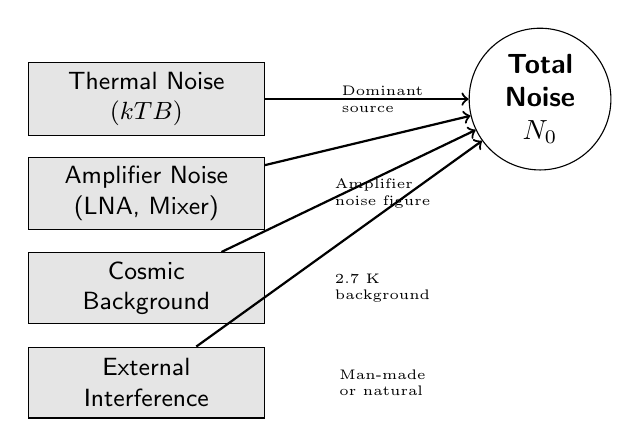
\begin{tikzpicture}[
  block/.style={rectangle, draw, minimum width=3cm, minimum height=0.9cm, font=\sffamily\small, align=center},
  node distance=1.2cm,
  font=\small
]
\node[block, fill=black!10] (thermal) {Thermal Noise\\$(kTB)$};
\node[block, below of=thermal, fill=black!10] (amp) {Amplifier Noise\\(LNA, Mixer)};
\node[block, below of=amp, fill=black!10] (cosmic) {Cosmic\\Background};
\node[block, below of=cosmic, fill=black!10] (interference) {External\\Interference};

\node[right of=thermal, node distance=5cm, circle, draw, minimum size=1.8cm, font=\bfseries\sffamily, align=center] (sum) {Total\\Noise\\$N_0$};

\draw[->,thick] (thermal) -- (sum);
\draw[->,thick] (amp) -- (sum);
\draw[->,thick] (cosmic) -- (sum);
\draw[->,thick] (interference) -- (sum);

% Annotations
\node[right of=thermal, node distance=3cm, font=\tiny, align=left] {Dominant\\source};
\node[right of=amp, node distance=3cm, font=\tiny, align=left] {Amplifier\\noise figure};
\node[right of=cosmic, node distance=3cm, font=\tiny, align=left] {2.7 K\\background};
\node[right of=interference, node distance=3cm, font=\tiny, align=left] {Man-made\\or natural};
\end{tikzpicture}
\end{center}

\textbf{Primary noise sources}:
\begin{itemize}
\item \textbf{Thermal noise (Johnson-Nyquist)}: Random electron motion in resistors
\item \textbf{Amplifier noise}: LNA and receiver front-end noise figure
\item \textbf{Cosmic background radiation}: 2.7~K microwave background
\item \textbf{External interference}: Man-made or natural (lightning, solar)
\end{itemize}

\subsubsection{Mathematical Model}

The total received signal with noise:
\begin{equation}
r(t) = \frac{s(t)}{\sqrt{L}} + n(t)
\end{equation}
where $n(t)$ is modeled as \textbf{Additive White Gaussian Noise (AWGN)}:
\begin{itemize}
\item \textbf{Gaussian}: Amplitude follows normal distribution $\mathcal{N}(0, \sigma^2)$
\item \textbf{White}: Flat power spectral density across all frequencies
\item \textbf{Zero mean}: $\mathbb{E}[n(t)] = 0$
\end{itemize}

\textbf{Thermal noise power}:
\begin{equation}
N = kTB
\end{equation}
where:
\begin{itemize}
\item $k = 1.38 \times 10^{-23}$ J/K (Boltzmann's constant)
\item $T$ = system noise temperature (Kelvin)
\item $B$ = bandwidth (Hz)
\end{itemize}

In dBm:
\begin{equation}
N\ [\text{dBm}] = -174 + 10\log_{10}(B) + 10\log_{10}\left(\frac{T}{290}\right)
\end{equation}
where $-174$ dBm/Hz is the thermal noise floor at room temperature (290~K).

\subsection{Combined Channel Model}

The complete channel model combines both effects in sequence:

\begin{center}
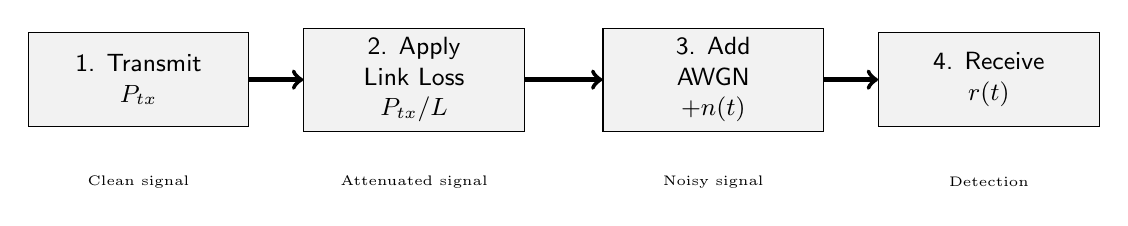
\begin{tikzpicture}[
  node distance=2.5cm,
  block/.style={rectangle, draw, minimum width=2.8cm, minimum height=1.2cm, font=\sffamily\small, align=center, fill=black!5},
  font=\small
]
\node[block] (tx) {1. Transmit\\$P_{\text{tx}}$};
\node[block, right of=tx, node distance=3.5cm] (loss) {2. Apply\\Link Loss\\$P_{\text{tx}}/L$};
\node[block, right of=loss, node distance=3.8cm] (noise) {3. Add\\AWGN\\$+n(t)$};
\node[block, right of=noise, node distance=3.5cm] (rx) {4. Receive\\$r(t)$};

\draw[->,ultra thick] (tx) -- (loss);
\draw[->,ultra thick] (loss) -- (noise);
\draw[->,ultra thick] (noise) -- (rx);

% Power annotations
\node[below of=tx, node distance=1.3cm, font=\tiny] {Clean signal};
\node[below of=loss, node distance=1.3cm, font=\tiny] {Attenuated signal};
\node[below of=noise, node distance=1.3cm, font=\tiny] {Noisy signal};
\node[below of=rx, node distance=1.3cm, font=\tiny] {Detection};
\end{tikzpicture}
\end{center}

\textbf{Step-by-step process}:
\begin{enumerate}
\item \textbf{Transmit}: Signal with power $P_{\text{tx}}$ is transmitted
\item \textbf{Attenuate}: Link loss reduces power to $P_{\text{tx}}/L$ where $L = 10^{L_{\text{dB}}/10}$
\item \textbf{Add noise}: AWGN with power $N = kTB$ is added
\item \textbf{Receive}: Final signal has power $P_{\text{rx}} = P_{\text{tx}}/L$ plus noise
\end{enumerate}

The resulting signal-to-noise ratio at the receiver:
\begin{equation}
\text{SNR} = \frac{P_{\text{rx}}}{N} = \frac{P_{\text{tx}}}{L \cdot kTB}
\end{equation}

In logarithmic form:
\begin{equation}
\text{SNR}_{\text{dB}} = P_{\text{tx}}\ [\text{dBm}] - L_{\text{dB}}\ [\text{dB}] - N\ [\text{dBm}]
\end{equation}

\section{Why Both Matter}

\subsection{Link Loss Affects Signal Power}

\begin{itemize}
\item High link loss (100+ dB) is typical in many systems
\item Reduces signal level but doesn't add randomness
\item Can be compensated with amplification (but amplifies noise too!)
\item Primarily determines required transmit power
\end{itemize}

\begin{warningbox}
\textbf{Amplification cannot overcome poor SNR.} Amplifying a weak signal also amplifies the noise proportionally. Link loss must be addressed at the system level through antenna gains, lower frequencies, or reduced distance---not just by amplification.
\end{warningbox}

\subsection{Noise Affects Signal Quality (SNR)}

\begin{itemize}
\item Adds random errors that can't be predicted or removed
\item Sets the fundamental limit on achievable BER
\item Can be improved with processing gain, error correction, or increased signal power
\item Determines required $E_b/N_0$ for target BER
\end{itemize}

\section{Link Budget and SNR Analysis}

The combination of link loss and noise determines receiver performance:
\begin{equation}
P_{\text{rx}}\ [\text{dBm}] = P_{\text{tx}}\ [\text{dBm}] - L_{\text{dB}}\ [\text{dB}]
\end{equation}
\begin{equation}
N\ [\text{dBm}] = -174 + 10\log_{10}(B) + NF
\end{equation}
\begin{equation}
\text{SNR}_{\text{dB}} = P_{\text{rx}}\ [\text{dBm}] - N\ [\text{dBm}]
\end{equation}
where $NF$ is the receiver noise figure in dB.

\subsection{Comparative Examples}

\begin{calloutbox}{Example 1: Good Link Budget}
\begin{itemize}
\item Transmit power: +30 dBm
\item Link loss: 100 dB
\item Received signal: \textbf{$-70$ dBm}
\item Noise floor: $-90$ dBm (1 MHz BW, 3 dB NF)
\item \textbf{Resulting SNR: 20 dB} ✓ \textbf{Excellent!}
\end{itemize}

\textbf{Analysis}: High SNR enables high-order modulation (16-QAM, 64-QAM) and achieves BER $< 10^{-6}$ easily.
\end{calloutbox}

\begin{calloutbox}{Example 2: Marginal Link Budget}
\begin{itemize}
\item Transmit power: +30 dBm
\item Link loss: 120 dB
\item Received signal: \textbf{$-90$ dBm}
\item Noise floor: $-90$ dBm
\item \textbf{Resulting SNR: 0 dB} ⚠ \textbf{Very challenging!}
\end{itemize}

\textbf{Analysis}: Only simple modulation (BPSK) viable. Requires FEC to achieve acceptable BER. Link margin is zero---no room for fading or interference.
\end{calloutbox}

\section{Worked Example: Complete Link Budget Analysis}

\textbf{Scenario}: Design a 2.4~GHz WiFi link over 100 meters with required BER $= 10^{-5}$ using BPSK modulation.

\subsection*{Given Parameters}

\begin{tabular}{@{}ll@{}}
Frequency & $f = 2.4$ GHz \\
Distance & $d = 100$ m \\
Data rate & $R_b = 1$ Mbps \\
Modulation & BPSK \\
Required BER & $10^{-5}$ \\
TX antenna gain & $G_t = 2$ dBi (omnidirectional) \\
RX antenna gain & $G_r = 2$ dBi (omnidirectional) \\
Cable losses & $L_c = 1$ dB (each side) \\
Implementation loss & $L_i = 2$ dB \\
Noise figure & $NF = 5$ dB \\
Temperature & $T = 290$ K (room temperature) \\
\end{tabular}

\subsection*{Step 1: Determine Required $E_b/N_0$}

For BPSK with BER $= 10^{-5}$:
\begin{equation}
\text{BER} = \frac{1}{2}\text{erfc}\left(\sqrt{\frac{E_b}{N_0}}\right) = 10^{-5}
\end{equation}

From tables or calculation: $(E_b/N_0)_{\text{required}} = 9.6$ dB

\textbf{Add implementation margin}: $3$ dB
\[
(E_b/N_0)_{\text{design}} = 9.6 + 3 = 12.6\ \text{dB}
\]

\subsection*{Step 2: Calculate Free-Space Path Loss}

Using the Friis equation:
\begin{equation}
L_{\text{FSPL}}\ [\text{dB}] = 20\log_{10}\left(\frac{4\pi d f}{c}\right)
\end{equation}
\begin{equation}
L_{\text{FSPL}} = 20\log_{10}\left(\frac{4\pi \times 100 \times 2.4 \times 10^9}{3 \times 10^8}\right) = 80.05\ \text{dB}
\end{equation}

\subsection*{Step 3: Calculate Total Link Loss}

\begin{align}
L_{\text{total}} &= L_{\text{FSPL}} - G_t - G_r + L_c + L_i \\
&= 80.05 - 2 - 2 + (1 + 1) + 2 \\
&= 80.05\ \text{dB}
\end{align}

\subsection*{Step 4: Calculate Noise Power}

Bandwidth for BPSK with $\alpha = 0.35$ roll-off:
\begin{equation}
B = R_b(1 + \alpha) = 1 \times 1.35 = 1.35\ \text{MHz}
\end{equation}

Thermal noise power:
\begin{equation}
N = kTB = (1.38 \times 10^{-23})(290)(1.35 \times 10^6) = 5.41 \times 10^{-15}\ \text{W}
\end{equation}

In dBm:
\begin{equation}
N\ [\text{dBm}] = 10\log_{10}(5.41 \times 10^{-15} / 10^{-3}) = -112.7\ \text{dBm}
\end{equation}

With noise figure:
\begin{equation}
N_{\text{total}} = -112.7 + 5 = -107.7\ \text{dBm}
\end{equation}

\subsection*{Step 5: Calculate Required Transmit Power}

From the $E_b/N_0$ requirement:
\begin{align}
\frac{E_b}{N_0} &= \text{SNR} \times \frac{B}{R_b} \\
\text{SNR}_{\text{dB}} &= (E_b/N_0)_{\text{dB}} - 10\log_{10}(B/R_b) \\
&= 12.6 - 10\log_{10}(1.35) = 12.6 - 1.3 = 11.3\ \text{dB}
\end{align}

Required received power:
\begin{equation}
P_{\text{rx}}\ [\text{dBm}] = N_{\text{total}} + \text{SNR}_{\text{dB}} = -107.7 + 11.3 = -96.4\ \text{dBm}
\end{equation}

Required transmit power:
\begin{equation}
P_{\text{tx}}\ [\text{dBm}] = P_{\text{rx}} + L_{\text{total}} = -96.4 + 80.05 = -16.4\ \text{dBm}
\end{equation}

Converting to linear scale:
\begin{equation}
P_{\text{tx}} = 10^{-16.4/10} \times 10^{-3} = 23\ \text{mW}
\end{equation}

\subsection*{Step 6: Link Margin Calculation}

Typical WiFi transmit power: $P_{\text{tx}} = +20$ dBm (100 mW)

\begin{equation}
\text{Link Margin} = P_{\text{tx,available}} - P_{\text{tx,required}} = 20 - (-16.4) = 36.4\ \text{dB}
\end{equation}

\begin{calloutbox}[colback=black!8!white,colframe=black]{Link Budget Summary}
\textbf{Result: Link closes with 36.4~dB margin}

This substantial margin accommodates:
\begin{itemize}
\item Multipath fading ($\sim$10--20 dB)
\item Interference and co-channel interference ($\sim$5--10 dB)
\item Obstacles (walls, furniture) ($\sim$5--15 dB)
\item Component aging and temperature variations ($\sim$2--3 dB)
\end{itemize}

\textbf{Conclusion:} Link is viable with significant margin for real-world impairments. 1~Mbps BPSK transmission at 100~m is easily achievable.
\end{calloutbox}

\section{Practical Applications}

\subsection{Satellite Communications}

Extreme link loss ($\sim$200 dB for GEO) dominates system design:

\begin{calloutbox}{GEO Satellite Downlink}
\begin{itemize}
\item \textbf{Challenge}: 36,000 km path loss = 205~dB at Ku-band
\item \textbf{Solution}: Large antennas (70~m DSN dishes), high TX power (200~W)
\item \textbf{Noise}: Deep space is quiet---cosmic background only
\item \textbf{Result}: Link closes with careful power budget management
\end{itemize}
\end{calloutbox}

\subsection{Cellular Networks}

Balanced link loss and noise considerations:

\begin{calloutbox}{LTE Cell Tower at 2~km}
\begin{itemize}
\item \textbf{Link loss}: $\sim$120 dB (including shadowing, building penetration)
\item \textbf{Noise}: Urban interference + thermal noise
\item \textbf{Strategy}: Dynamic power control, adaptive modulation (QPSK to 256-QAM)
\item \textbf{Trade-off}: High SNR near tower = high throughput; low SNR at edge = robust low-rate modes
\end{itemize}
\end{calloutbox}

\subsection{Deep-Space Probes}

Ultimate challenge---both extreme link loss and low power:

\begin{calloutbox}{Voyager 1 at 24 Billion km}
\begin{itemize}
\item \textbf{Link loss}: $\sim$310 dB (interstellar distance)
\item \textbf{TX power}: 23~W (RTG power source, degrading over time)
\item \textbf{Data rate}: 160 bps (originally 115 kbps in 1980s)
\item \textbf{FEC}: Concatenated coding (gain $\sim$10 dB) essential
\item \textbf{Key insight}: Every 0.1~dB matters at this extreme
\end{itemize}
\end{calloutbox}

\subsection{WiFi and WLAN}

Moderate link loss, variable noise environment:

\begin{calloutbox}{WiFi in Office Building}
\begin{itemize}
\item \textbf{Link loss}: 60--100 dB (depending on walls, floors)
\item \textbf{Noise}: High interference (2.4 GHz ISM band is crowded)
\item \textbf{Strategy}: Rate adaptation algorithms (adjust modulation/coding based on SNR)
\item \textbf{Challenge}: Noise often dominates over path loss in dense deployments
\end{itemize}
\end{calloutbox}

\section{Key Insights and Trade-offs}

\begin{keyconcept}
\textbf{The fundamental relationship}:
\[
\text{More TX Power} \rightarrow \text{Overcomes Link Loss} \rightarrow \text{Higher RX Power} \rightarrow \text{Better SNR} \rightarrow \text{Lower BER}
\]

However, practical limits exist:
\begin{itemize}
\item \textbf{TX power}: Battery life, regulatory limits, PA efficiency
\item \textbf{RX sensitivity}: Thermal noise floor, amplifier noise figure
\item \textbf{System cost}: Larger antennas, better LNAs increase cost
\item \textbf{Interference}: More TX power creates interference for others
\end{itemize}
\end{keyconcept}

\subsection{Design Trade-offs}

\begin{center}
\begin{tabular}{@{}lll@{}}
\toprule
\textbf{Parameter} & \textbf{Improves} & \textbf{Cost/Limitation} \\
\midrule
Increase TX power & Link budget & Battery, regulations, interference \\
Larger antennas & Link budget & Size, weight, cost, pointing \\
Lower frequency & Path loss & Spectrum availability, antenna size \\
Narrower bandwidth & Noise power & Data rate reduced \\
Better LNA & Noise figure & Cost, power consumption \\
FEC coding & Effective SNR & Latency, bandwidth overhead \\
\bottomrule
\end{tabular}
\end{center}

\section{Summary}

\begin{center}
\begin{tabular}{@{}lll@{}}
\toprule
\textbf{Aspect} & \textbf{Link Loss} & \textbf{Noise} \\
\midrule
Nature & Deterministic & Random (stochastic) \\
Effect & Multiplicative & Additive \\
Predictability & Calculable & Statistical \\
Mitigation & Antenna gain, TX power & Reduce bandwidth, FEC \\
Amplification & Helps if before RX & Amplified with signal \\
Typical range & 60--310 dB & $-174$ dBm/Hz (thermal) \\
Primary impact & Power budget & BER performance \\
\bottomrule
\end{tabular}
\end{center}

\textbf{Key relationships}:
\begin{itemize}
\item $\text{SNR} = (P_{\text{tx}} - L_{\text{dB}}) - N$
\item Both link loss and noise must be managed for reliable communication
\item High link loss requires high TX power or high antenna gains
\item High noise requires wide margins (higher SNR) or robust modulation/coding
\item The product $L \times N$ determines required transmit power for given BER
\end{itemize}

\section{Further Reading}

\draw[->,thick] (tx) -- (loss);
\draw[->,thick] (loss) -- (rx);
\draw[->,thick] (rx) -- (snr);
\draw[->,thick] (snr) -- (ber);
\end{tikzpicture}
\end{center}

\textbf{Practical limits:}
\begin{itemize}
\item \textbf{Chapter 4:} Signal-to-Noise Ratio (SNR)---detailed SNR analysis
\item \textbf{Chapter 5:} Additive White Gaussian Noise (AWGN)---noise modeling
\item \textbf{Chapter 11:} Free-Space Path Loss---propagation fundamentals
\item \textbf{Chapter 15:} Bit Error Rate (BER) Performance---error analysis
\item \textbf{Chapter 18:} Link Budget Analysis---complete system design
\item \textbf{Chapter 22:} Forward Error Correction---coding for noise mitigation
\item \textbf{Chapter 25:} Antenna Fundamentals---antenna gains and patterns
\end{itemize}
